\hypertarget{adroit-pen-ux73afux5883ux89c2ux6d4bux52a8ux4f5cux4e0eux6210ux529fux6307ux6807}{%
\section{Adroit Pen 环境、观测、动作与成功指标}\label{adroit-pen-ux73afux5883ux89c2ux6d4bux52a8ux4f5cux4e0eux6210ux529fux6307ux6807}}

\hypertarget{ux73afux5883ux4e0eux52a8ux4f5cux63a5ux53e3}{%
\subsection{环境与动作接口}\label{ux73afux5883ux4e0eux52a8ux4f5cux63a5ux53e3}}

实验固定使用 \texttt{AdroitHandPen-v1} 的 dense-reward 配置。\par 数据集为 Minari 提供的 \texttt{D4RL/pen/human-v2}。episode horizon 为 200，动作维度为 24；actor 输出统一映射到环境动作范围。主要环境版本是 Python 3.11.15、Gymnasium 0.29.1、Gymnasium-Robotics 1.2.3、Minari 0.5.3、MuJoCo 2.3.7、NumPy 1.26.4 和 PyTorch 2.8.0+cu128。渲染使用 EGL、84×84 RGB、固定 camera id \texttt{-1}，相机参数为 distance 1.0、azimuth −45°、elevation −25°、lookat \texttt{{[}0,\ -0.2,\ 0.22{]}}。

Oracle actor 使用官方 45 维完整 observation，包括手部状态、物体和目标的仿真真值。初始视觉 actor 的部署输入是 4-frame RGB history、\texttt{qpos{[}:24{]}}、\texttt{qvel{[}:24{]}} 和 previous action；最终 E2 使用 8-step 因果 RGB、同样可部署的 proprioception 与 executed-action history。训练阶段可以用 simulator state 做监督，但 E2 推理路径不会读取笔的位置、速度、姿态、目标真值或其他 privileged state。

\hypertarget{ux6210ux529fux7387ux548cux4fddux6301ux6307ux6807}{%
\subsection{成功率和保持指标}\label{ux6210ux529fux7387ux548cux4fddux6301ux6307ux6807}}

\textbf{Benchmark success} 与环境 \texttt{info{[}"success"{]}} 兼容：episode 任意时刻进入官方目标条件即计为成功。它回答``策略有没有到过目标''，但不保证之后仍然稳定。

\textbf{Strict success} 要求 episode 最后连续 20 steps 都满足官方目标条件，同时笔未掉落，state/action 中没有 non-finite 数值。它更接近``完成后稳定保持''的项目目标，因而是与 Benchmark 并列报告的核心指标。

为理解成功结构，报告还使用三个诊断量：

\begin{itemize}
\tightlist
\item
  \textbf{Goal entry}：episode 是否至少一次进入目标区域；在当前实现中与 Benchmark 的事件口径一致。
\item
  \textbf{Exit after entry}：已经 entry 的 episode 中，之后再次退出目标区域的比例。
\item
  \textbf{20-step hold}：episode 内是否出现至少连续 20 步处于目标区域的窗口。
\end{itemize}

需要特别注意，Exit/Entry 是条件比例，分母取决于策略自己的 entry 数。若一个策略很少进入目标，exit ratio 可能看上去较低，却不代表保持能力更强。D1 就出现了这类 acquisition--hold 反向移动。因此它只用于诊断，不能替代 Benchmark、Strict 或共同 root 的 fixed-entry survival。

\textbf{Fixed-entry hold} 从同一批 E0 first-entry simulator roots 恢复多个策略，比较从完全相同状态起始后的 20-step 和 50-step survival。它控制了``谁先进入、进入了多少次''的差异，更接近对保持能力的共同状态诊断；但它仍然是仿真恢复实验，不等价于整条闭环 episode 指标。

\hypertarget{ux8badux7ec3ux4e0eux8bc4ux6d4bux6570ux636eux8d26ux672c}{%
\subsection{训练与评测数据账本}\label{ux8badux7ec3ux4e0eux8bc4ux6d4bux6570ux636eux8d26ux672c}}

\begin{longtable}[]{@{}
  >{\raggedright\arraybackslash}p{(\columnwidth - 6\tabcolsep) * \real{0.2000}}
  >{\raggedleft\arraybackslash}p{(\columnwidth - 6\tabcolsep) * \real{0.2667}}
  >{\raggedright\arraybackslash}p{(\columnwidth - 6\tabcolsep) * \real{0.2000}}
  >{\centering\arraybackslash}p{(\columnwidth - 6\tabcolsep) * \real{0.3333}}@{}}
\toprule\noalign{}
\begin{minipage}[b]{\linewidth}\raggedright
数据
\end{minipage} & \begin{minipage}[b]{\linewidth}\raggedleft
规模
\end{minipage} & \begin{minipage}[b]{\linewidth}\raggedright
用途
\end{minipage} & \begin{minipage}[b]{\linewidth}\centering
是否进入最终 E2 训练
\end{minipage} \\
\midrule\noalign{}
\endhead
\bottomrule\noalign{}
\endlastfoot
Human demonstrations & 25 episodes、4,975 transitions & BC、critic warm-up、offline AWAC & 基础控制器 \\
State-distillation source & 544 simulation episodes、108,800 transitions & E1/E2 时序状态估计 & 是 \\
D1 student-visited data & 300 episodes、60,000 transitions & 仅训练 D1 & 否 \\
V4/V5 branch data & 240 roots / 1,200 roots 的反事实候选实验 & 失败机制分析 & 否 \\
Confirmation & 300 episodes & 独立 paired 评测 & 否 \\
Fixed-entry hold & 200 common roots & 共同状态 hold 诊断 & 否 \\
3-seed evaluation & 3 个 recipe seed，各评同一组 100 states & 配方复现 & 否 \\
Frozen test & 200 episodes & 一次性最终测试 & 否 \\
\end{longtable}

\begin{figure}
\centering
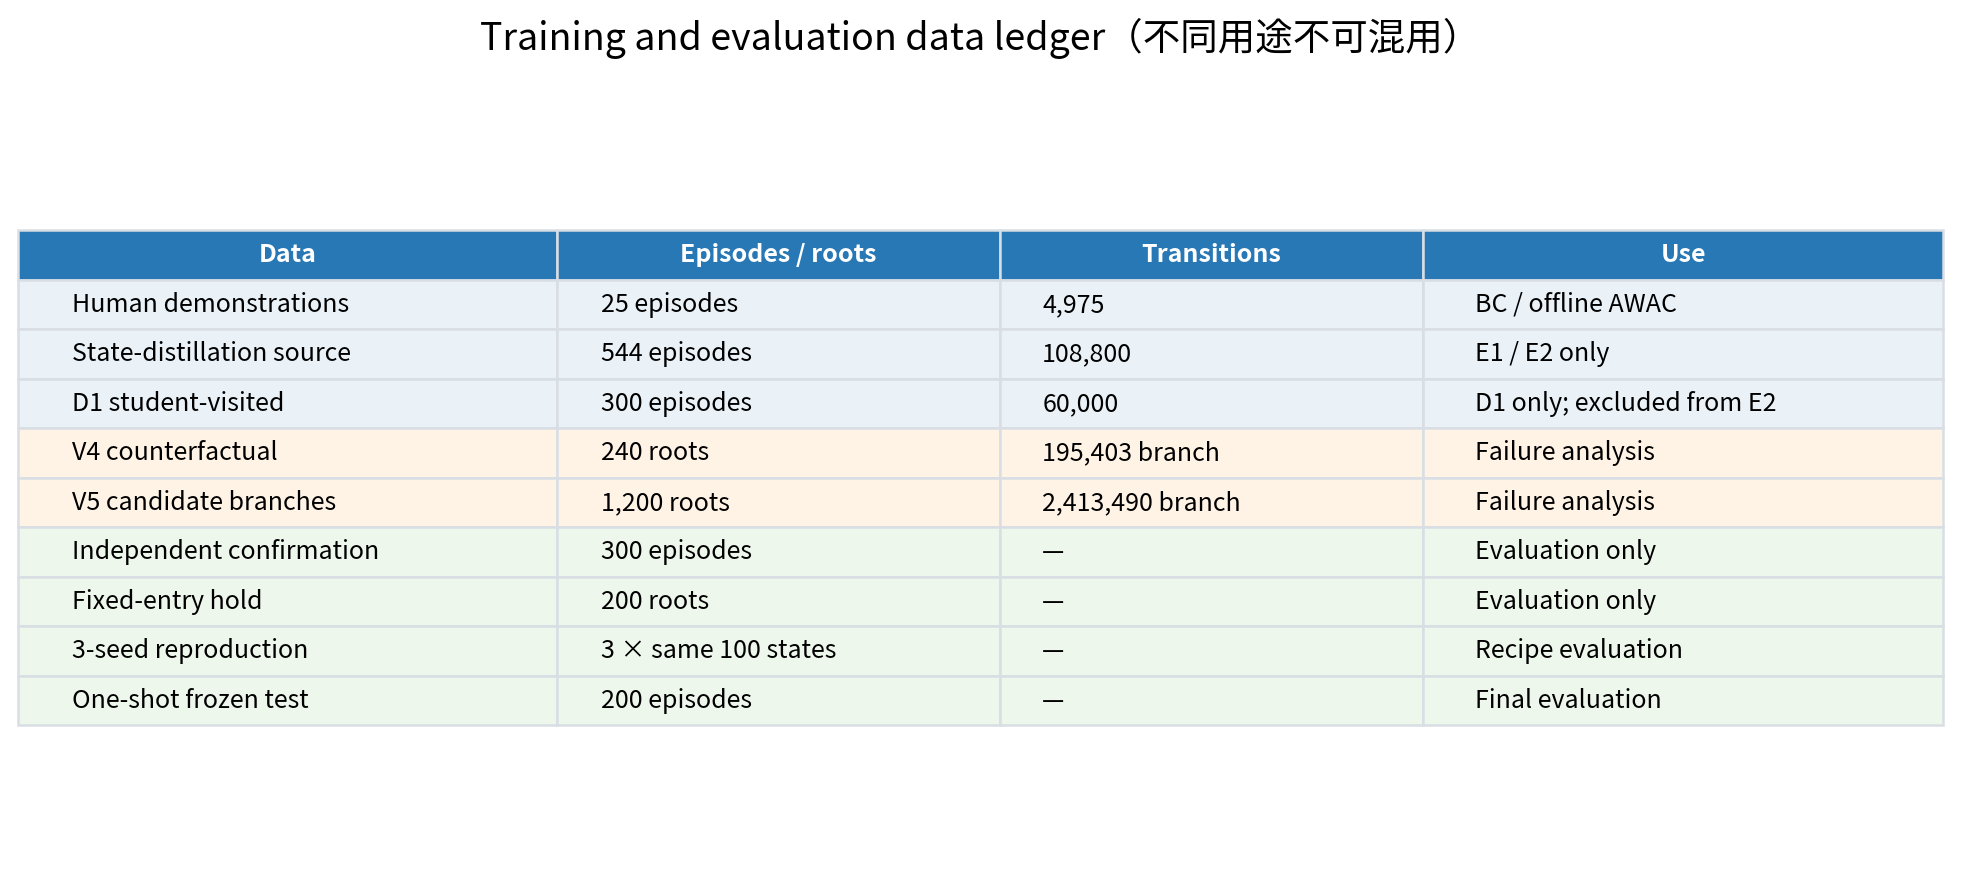
\includegraphics[width=\linewidth]{figures/02_data_ledger.png}
\caption{训练与评测数据账本}
\end{figure}

\textbf{图 2｜训练与评测数据账本。} Human demo、state-distillation source、D1 数据、反事实 branch 数据和评测 bank 用途互不替换。3-seed 的三个模型使用相同 100 个 evaluation states，因此不能把它们当作 300 个独立初始状态计算普通 pooled binomial CI；confirmation 与 frozen test 则是独立于训练的数据。

544 条 state-distillation 轨迹由两部分构成：已有 V4 training rollout 的 244 episodes，加上新采集的 300 条 Frozen Oracle simulation episodes，共 108,800 个长度为 200 的稠密时序样本。D1 额外访问 300 episodes、60,000 transitions，但仅用于 D1 实验，不能倒算进已冻结的 E2 训练集。V4/V5 的 branch rollout 用于判断局部动作修正是否可行，也没有进入 E2。

\textbf{本章结论。} 报告同时衡量``到达''和``保持''，并把条件性 exit 指标与共同 root 的 hold 诊断分开。最终 E2 是部署时只读取 RGB、proprioception 和动作历史的视觉策略，但其训练数据明显超过 25 条 human demo，任何结果解读都必须保留这一区别。

\autocite{gymnasiumrobotics2024,minari2024}
